\chapter{Getting started with OpenIMAJ using Maven}
\pagestyle{headings}
\pagenumbering{arabic}
Apache Maven is a project management tool. \marginpar{You can find out more 
about Apache Maven at \url{http://maven.apache.org}.} Maven performs tasks such 
as automatic  dependency management, project packaging and more. We \textbf{strongly} 
encourage anyone using OpenIMAJ to use Maven to get their own project started. 
We've even provided a Maven \textbf{archetype} for OpenIMAJ (basically a project template) 
that lets you get started programming with OpenIMAJ quickly. 

OpenIMAJ requires Maven 3. You can check if you have Maven installed already 
by opening a terminal (or DOS command prompt) and typing:
\begin{lstlisting}[language=bash]
mvn -version
\end{lstlisting}
If Maven is found the, version will be printed. If the version is less than 3.0, 
or Maven was not found, go to \url{http://maven.apache.org} to download and 
install it. Once you've installed Maven try the above command to test that it 
is working.

To create a new OpenIMAJ project, run the following command (note that the command is all on one line and there is no space between \verb+maven.openimaj.org/+ and \verb+archetype-catalog.xml+):
\begin{lstlisting}[language=bash]
mvn -DarchetypeCatalog=http://maven.openimaj.org/archetype-catalog.xml archetype:generate
\end{lstlisting}

Maven will then prompt you for some input. \marginpar{Versions of the archetype after 1.0.5 automatically select the corresponding OpenIMAJ version. With all versions of the archetype, you can override this by setting the \texttt{openimajVersion} on the command-line with the \texttt{-D} argument.} Firstly, when prompted, choose 
the \texttt{openimaj-quickstart-archetype} and choose the latest version. For the \verb+groupId+, 
enter something that identifies you or a group that you belong to (for example, I might choose 
\verb+uk.ac.soton.ecs.jsh2+ for personal projects, or \verb+org.openimaj+ for OpenIMAJ sub-projects). 
For the \verb+artifactId+ enter a name for your project (for example, \verb+OpenIMAJ-Tutorial01+). The 
version can be left as \verb+1.0-SNAPSHOT+, and the default package is also OK. Finally enter \verb+Y+ and press return
to confirm the settings. Maven will then generate a new project in a directory with the same 
name as the \verb+artifactId+ you provided.

The project directory contains a file called \verb+pom.xml+ and a directory called \verb+src+. 
%\marginpar{The \texttt{pom.xml} file created by the \texttt{openimaj-quickstart-archetype} includes
%all the main OpenIMAJ library dependencies, as well as a configuration for the maven assembly 
%plugin.}
The \verb+pom.xml+ file describes all of the dependencies of the project and also contains 
instructions for packaging the project into a fat jar that contains all your project code and 
resources together with the dependencies. If you find that you need to add another library to 
your project, you should do so by editing the \verb+pom.xml+ file and adding a new dependency. 
The \verb+src+ directory contains the code for your project. In particular, \verb+src/main/java+ 
contains your java application code and \verb+src/test/java+ contains unit tests.

The default project created by the archetype contains a small ``hello world'' application. To 
compile and assemble the ``hello world'' application you \verb+cd+ into the project directory from the command line (replacing \verb+OpenIMAJ-Tutorial01+ with the name of your project):
\begin{lstlisting}[language=bash]
cd OpenIMAJ-Tutorial01
\end{lstlisting}
and run the command:
\begin{lstlisting}[language=bash]
mvn assembly:assembly
\end{lstlisting}
This will create a new directory called target that contains the assembled application jar 
(the assembled jar is the one whose name ends with -jar-with-dependencies.jar). To run the 
application, enter: 
\begin{lstlisting}[language=bash]
java -jar target/OpenIMAJ-Tutorial01-1.0-SNAPSHOT-jar-with-dependencies.jar
\end{lstlisting}
The application will then run, and a window should open displaying a picture with the text 
\marginpar{
\includegraphics[width=\marginparwidth]{hello-world.png}}
``hello world''. Closing the window, or ctrl-c on the command line, will quit the application.

\section*{Integration with your favourite IDE}
We could now go ahead and start playing with the code in a text editor, however this really 
isn't recommended! Using a good Integrated Development Environment (IDE) with auto-completion will 
make your experience much better.

Maven integrates with all the popular IDEs. The OpenIMAJ developers all use Eclipse 
(\url{http://www.eclipse.org}) so that is what we're most familiar with, however we should be able 
to help getting it set up in a different IDE if you wish. 

Integration with Eclipse is quite simple. From the command line, inside the project directory, 
issue the command:
\begin{lstlisting}[language=bash]
mvn eclipse:eclipse
\end{lstlisting}
This will generate Eclipse project files in the same directory. In Eclipse you can then import 
the project into the Eclipse workspace (File>import..., choose ``Existing projects into workspace'', 
select the project directory, make sure ``Copy projects into workspace'' is \textbf{unchecked}, then click
 ``Finish''). The project should then appear in the workspace and you'll be able to look at the 
App.java file that was generated by the archetype.

\textbf{IMPORTANT} By default Eclipse doesn't know about Maven and its repositories of jars. When you 
first import an OpenIMAJ project into Eclipse it will have errors. You can fix this by adding 
a new Java classpath variable (\verb+Eclipse>Preferences>Java>+ \verb+Build Path>Classpath Variables+) 
called \verb+M2_REPO+. The value of this variable is the location of your \verb+.m2/repository+ directory. 
\marginpar{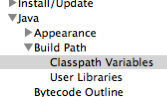
\includegraphics[width=\marginparwidth]{classpath.png}}
For Unix systems this is usually found in your home directory, for Windows systems it is found 
in \verb+C:\Documents and+ \verb+Settings\<user>\+.

Once you've opened the \verb+App.java+ file in Eclipse, you can right-click on it and select 
\verb+Run as>Java Application+ to run it from within Eclipse. 
\marginpar{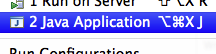
\includegraphics[width=\marginparwidth]{runas2.png}}

\section*{Exercises}
\subsection{Exercise 1: Playing with the sample application}
Take a look at the App.java from within your IDE. Can you modify the code to render something 
other than ``hello world'' in a different font and colour?
